\chapter{図表を載せる}
図\ref{fig:sin}のように参照できる.
同様に表\ref{tab:demo}のように参照できる.

\begin{figure}[h]
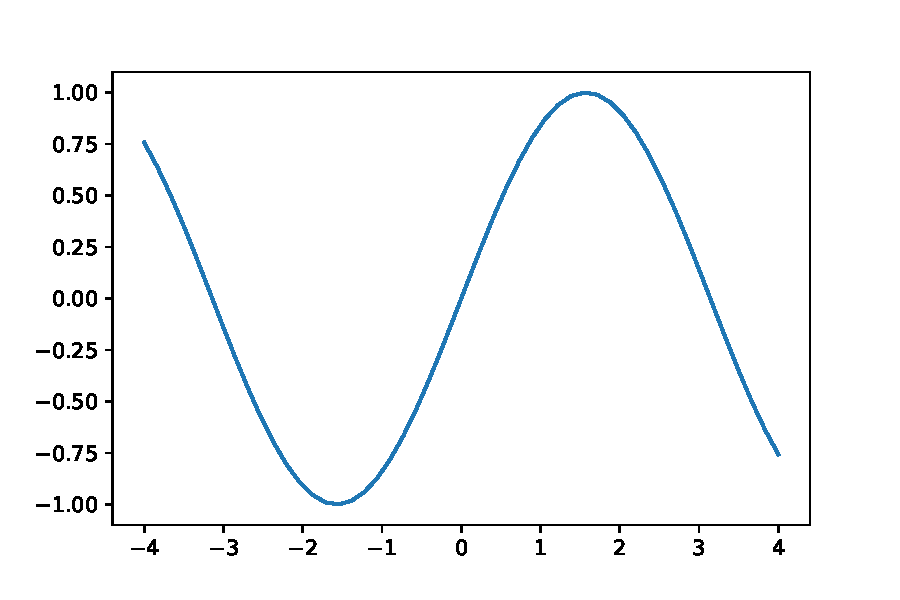
\includegraphics[scale=0.8]{figures/sample-figure.pdf}
\centering
\caption{正弦波}
\label{fig:sin}
\end{figure}

\begin{table}[h]
\centering
\caption{サンプル}
\label{tab:demo}
\begin{tabular}{@{}llr@{}}
\toprule
\multicolumn{2}{c}{Item} &            \\ \cmidrule(r){1-2}
Animal     & Description & Price (\$) \\ \midrule
Gnat       & per gram    & 13.65      \\
           & each        & 0.01       \\
Gnu        & stuffed     & 92.50      \\
Emu        & stuffed     & 33.33      \\
Armadillo  & frozen      & 8.99       \\ \bottomrule
\end{tabular}
\end{table}
